\documentclass[a4paper,12pt,oneside,bibtotoc,numbers=noenddot]{scrreprt}

%Pakete
\usepackage[latin9]{inputenc}
\usepackage[ngerman]{babel}
\usepackage{listings}
\usepackage{graphicx}
\usepackage{BachelorThesis}

% Allgemeine Informationen
\newcommand\mytitle{Titel der Arbeit}
\newcommand\myauthor{Name des Autors oder der Autoren}
\newcommand\mydepartment{Informatik und Elektrotechnik}
\newcommand\myinstitute{Hochschule Zittau/G\"{o}rlitz}
\newcommand\mytutor{Name und Titel des betreuenden Professors}
\newcommand\mySecondTutor{Name und Titel des betrieblichen Betreuers}

% Abstracts
\newcommand\mysubject{Das deutsche Abstract.}
\newcommand\mysubjectenglish{The english abstract.}

% PDF-Einstellungen
\hypersetup
{
	pdftitle = \mytitle,
	pdfsubject = \mysubject,
	pdfauthor = \myauthor,
	pdfkeywords = {},
	colorlinks = {true},
	pdfborder = 0 0 0
}

\begin{document}
\nocite{*}

%
\pagenumbering{alph}
\begin{titlepage}
\thispagestyle{empty} 
 \begin{center}
 \vspace{2.0cm} 
 {\bfseries \huge Verse des Alten Testaments clustern\\}
 \vspace{3.0cm} 
 {\bfseries \huge Belegarbeit\\}
 \vspace{3.0cm}
 {\normalsize eingereicht am Fachbereich\\}
 {\bfseries \Large Informatik\\}
 {\normalsize der Hochschule Zittau/G�rlitz (HAW)\\}
 \vspace{1cm}
 {\normalsize als Pr�fungsleistung im Fach\\}
 {\bfseries \Large Data Mining\\}
 \vspace{1cm}
 {\normalsize vorgelegt von:\\}
 {\bfseries \Large Christof Ochmann (35989)\\
 Ingo K�rner (40586)\\}
 \vspace{1cm}
 {\normalsize  G�rlitz, 11. Juli 2012\\}
 \vspace{0.5cm}
 Betreuer:	Prof. ten Hagen\\
 \vfill
\end{center}
\end{titlepage}

%
%% Kurzreferat
\thispagestyle{empty}
\section*{Abstract}\label{Abstract}
In diesem Projekt werden die Verse des Alten Testaments geclustert. Einander �hnliche Verse sollen durch Clusteralgorithmen in das selben Cluster gruppiert werden. Es wird untersucht, bei wie vielen Attributen und wie vielen Clustern die besten Resultate erzielt werden. Der Clusteralgorithmus soll dabei auf einem handels�blichen Laptop ausgef�hrt werden. Verteiltes Clustern ist nicht Gegenstand dieser Arbeit.


%\mysubject
%\section*{Abstract}
%\mysubjectenglish

\pagenumbering{Roman}
\tableofcontents
\listoffigures
%\lstlistoflistings

\begin{listofacronyms}
\acronym{AT}{Altes Testament}
\acronym{ARFF}{Attribute-Relation File Format}
\acronym{JVM}{Java Virtual Machine}
\acronym{EM}{Expectation Maximisation}

\end{listofacronyms}

\begin{flushleft}
\begin{thebibliography}{sotief}
\bibitem{bib1}{Martin, Robert C. (2008): Clean Code: A Handbook of Agile Software Craftsmanship. Prentice Hall International}

\bibitem{bib2}{Freeman, Eric (2007): Entwurfsmuster von Kopf bis Fu�. O'REILLY}

\bibitem{bib3}{\begin{verbatim}http://www.cs.waikato.ac.nz/ml/weka/arff.html (08.06.2012)\end{verbatim}} 

\bibitem{bib4}{\begin{verbatim}http://wiki.pentaho.com/display/DATAMINING (08.06.2012)\end{verbatim}} 




\end{thebibliography}
\end{flushleft}

\newpage
\pagestyle{chapterStyle}
\pagenumbering{arabic}

\chapter{Theorie}
\section{Einleitung}\label{Einleitung}

\section{Aufgabenstellung}\label{Aufgabenstellung}
Durch Clustering werden �hnlichkeiten in gro�en Datenbest�nden gefunden. In diesem Projekt werden mit Hilfe von Clustering-Algorithmen Verse des AT geclustert. Dabei sollen einander �hnliche Verse in einem Clustern zusammenfasst werden, d.h. Datens�tze, die sich �hneln, kommen in dasselbe Cluster. In diesem Projekt werden verschiedene Clusteralgorithmen auf das Alte Testament angewendet. In Werkzeugen wie Weka oder ELKI sind diese Algorithmen bereits implementiert und k�nnen genutzt werden.
Es soll nur auf einer Maschine geclustert werden, d.h. skalierbares Datamining mit Apache Mahout wird in dieser Arbeit nicht behandelt.
\section{Relevanz des Forschungsgegenstandes}\label{RelevanzDesForschungsgegenstandes}

\section{Der aktuelle Wissensstand}\label{DerAktuelleWissensstand}

\section{Testrechner}\label{Testrechner}
Der Testrechner besteht aus einem Laptop mit einem 64 Bit Dual Core Prozessor von AMD mit 2.1 GHz und 8GB RAM.
\section{Der Aufbau des Alten Testaments}\label{AufbauAT}
Jeder Vers des AT steht in einer eigenen Zeile, unabh�ngig, ob der Vers eher kurz ist, wie
"`Am Anfang schuf Gott Himmel und Erde."'

oder eher lang ist wie:
"`Da wurden berufen des K�nigs Schreiber zu der Zeit im dritten Monat, das ist der Monat Sivan, am dreiundzwanzigsten Tage, und wurde geschrieben, wie Mardochai gebot, an die Juden und an die F�rsten, Landpfleger und Hauptleute in den Landen von Indien bis an das Mohrenland, n�mlich hundert und siebenundzwanzig L�nder, einem jeglichen Lande nach seiner Schrift, einem jeglichen Volk nach seiner Sprache, und den Juden nach ihrer Schrift und Sprache."'

Die Zeilennummer identifiziert somit einen Vers eindeutig.

Neben den Versen gibt es auch noch Kapitel�berschriften wie z.B. "`Kapitel 1"' und Buchnamen wie z.B. "`1. Buch Mose"', die auch eine eindeutige Zeilennummer haben. Zur Vereinfachung wird auch bei Buchnamen und Kapiteln von Versen gesprochen. Die Verse eines Buches im AT sind zwar auch durchnummeriert, diese Nummerierung wird aber ignoriert, da sie nur innerhalb eines Kapitels eindeutig ist.
\begin{figure}[htp]
\centering
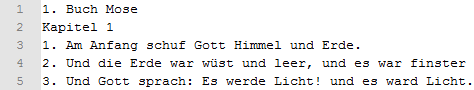
\includegraphics[width=1\textwidth]{Ingo/Bilder/AufbauAT.png}
\caption{Aufbau des AT}
\label{fig:AufbauAT}
\end{figure}
\section{ARFF}\label{ARFF}
Damit die Clusteralgorithmen auf das AT angewandt werden k�nnen, muss das AT vorher in das ARFF-Format (Attribute-Relation File Format) umgewandelt werden.

ARFF (Attribute-Relation File Format) ist eine Textdatei, die eine Liste von Instanzen beschreibt, die sich eine Menge von Attributen teilen. Eine Instanz w�re in unserem Beispiel ein Vers des AT. Die Attribute, die sich ein Vers mit anderen Versen teilt, sind die W�rter aus denen der Vers besteht.
Der Vers "`1. Am Anfang schuf Gott Himmel und Erde."' besteht aus der Attribut-Menge {1, Am, Anfang, schuf, Gott, und, Erde, Himmel}

Die Elemente "`1"', "`Himmel"', "`und"', "`Erde"' teilt sich der Vers z.B. mit dem Vers "`1. Also ward vollendet Himmel und Erde mit ihrem ganzen Heer."'

Man kann sagen, dass diese zwei Instanzen bzw. Verse deswegen eine gewissen �hnlichkeit haben, da sie sich einige gemeinsame Attribute teilen.

Eine ARFF-Datei besteht aus zwei Teilen. Dem Header- und dem Data-Teil. Im Header-Teil befinden sich die Attribute. Zu beachten ist, dass es sich bei dem Wert eines Attributes um die H�ufigkeit handelt, wie oft das Attribut im Vers vorkommt. Jedes Attribute hat einen Datentyp. Im vorliegenden Fall handelt es sich um Zahlen.
Im Datenteil befinden sich die Instanzen, d.h. die Verse. Sie bestehen aus den H�ufigkeiten, die mit Komma getrennt sind. Eine Instanz im Datenteil hat so viele mit Komma getrennte Zahlen, wie es Attribute im Header gibt. Jede Zahl steht f�r ein Attribut im Header. Die Position eines Attributes im Header stimmt mit der Position des Attributes in der Instanz �berein. D.h. das die dritte Zahl einer Instanz f�r das Attribut "`Anfang"' steht, da dieses auch an dritter Position im Header auftaucht.

Im folgenden sind drei Verse gegeben:

1. Buch Mose \\
Kapitel 1 \\
1. Am Anfang schuf Gott Himmel und Erde. \\

F�r diese drei Verse werden zehn Attribute definiert:

\% 1. Title: AT
@RELATION AT \\

@ATTRIBUTE 1 NUMERIC \\
@ATTRIBUTE Am NUMERIC \\
@ATTRIBUTE Anfang NUMERIC \\
@ATTRIBUTE schuf NUMERIC \\
@ATTRIBUTE Gott NUMERIC \\
@ATTRIBUTE Himmel NUMERIC \\
@ATTRIBUTE und NUMERIC \\
@ATTRIBUTE Erde NUMERIC \\
@ATTRIBUTE Fluss NUMERIC \\
@ATTRIBUTE Feld NUMERIC \\

Im Daten-Teil wird jeder Vers durch eine Instanz ausgedr�ckt. Die Instanz hat soviele Zahlen wie es Attribute im Header-Teil gibt. Eine 0 bedeutet, das Attribut kommt im Vers nicht vor. Eine 1 bedeutet, das Attribut kommt im Vers einmal vor.

@DATA \\
1,0,0,0,0,0,0,0,0,0 \\
1,0,0,0,0,0,0,0,0,0 \\
1,1,1,1,1,1,1,1,0,0 \\


\section{Clustering-Verfahren}\label{Clustering}
Ziel des Clustering ist es in Datenbest�nden Objekte zu finden, die m�glichst �hnlich sind, um diese anschlie�end in Gruppen(Cluster) zu untergliedern. Im Gegensatz zur Klassifikation werden Daten nicht bestehenden Klassen zugeordnet, sondern neue Gruppen m�ssen identifiziert werden. Die gefundenen Gruppen k�nnen sp�ter beispielsweise zur Mustererkennung, automatisierten Klassifizierung oder Marktsegmentierung verwendet werden. Die Clustering-Verfahren lassen sich in partitionierende, hierarchische, graphentheoretische, optimierende sowie in weitere Unterverfahren einteilen. \\
\begin{enumerate}
\item \textbf{Partitionierende Verfahren} \\
Bei den partitionierenden Verfahren ist die Anzahl der Cluster am Anfang festgelegt und es werden keine zus�tzlichen Gruppen gebildet. Die Prozesse beginnen immer mit einer vorgegebenen Anfangspartition und die einzelnen Objekte werden iterativ von einer Klasse in eine andere verschoben. Dabei wird ein gew�hltes Kriterium schrittweise optimiert, wie beispielsweise die Distanz zwischen Objekten. Die partitionierende Verfahren kann man in zwei Kategorien einteilen:
\begin{enumerate}
\item \textbf{Austauschverfahren mit Zielfunktion}(Hill-climbing methods) \\
 Die Anfangspartition wird gem�� eines G�tekriteriums iterativ durch Umgruppierung der Objekte verbessert. Bei jedem Objekt wird �berpr�ft, ob eine Verschiebung in eine andere Klasse das G�tekriterium verbessert oder nicht. Als G�tekriterium verwendet man bei Clusteranalysen h�ufig das Varianzkriterium. Weitere in Frage kommenden Kriterien sind das Spurkriterium oder das Determinantenkriterium.
\item \textbf{Minimaldistanz-Verfahren} \\
Die Anfangspartition wird bei diesem Verfahren iterativ verbessert indem jedes Objekt der Klasse hinzugef�gt wird, zu deren Klassenzentroid es die geringste euklidische Distanz hat. Beendet wird das Verfahren wenn keine Verschiebung von Objekten mehr stattfindet.
\end{enumerate}
\end{enumerate}

\subsection{Minimaldistanz-Verfahren}\label{Minimaldistanz}
\begin{enumerate}
\item \textbf{k-Means-Verfahren} \\
Eine gute und bekannte Clustering-Methode in der Kategorie der Minimaldistanzverfahren ist das k-Means-Verfahren. Dabei wird ebenfalls die euklidische Distanz herangezogen mit dem Unterschied, dass nach jedem Klassenwechsel die Klassenzentroide neu berechnet werden und dieses Verfahren gegen ein lokales Optimum konvergiert. Beendet wird das k-Means-Verfahren wenn z-mal hintereinander keine Objekte mehr verschoben wurden, und somit jedes Objekt zu seinem Klassenzentroid den geringsten euklidischen Abstand im Vergleich zu anderen Klassen aufweist. Der Nachteil dieser Methode ist, dass die L�sung von der Reihefolge der Iterationen abh�ngt und nicht nur von der Anfangspartition, au�erdem k�nnen Ausrei�er nicht erkannt werden.
\item \textbf{EM-Algorithmus}(Expected Maximization)
Der EM-Algorithmus ist ein effizientes und iteratives Verfahren zur Maximum-Likelihood-Sch�tzung und eignet sich sehr gut f�r die Durchf�hrung der ML-Sch�tzung mit fehlenden oder versteckten Daten. 
Der EM-Algorithmus wird auch als Clusterverfahren eingesetzt. Zu Beginn des Vorgangs wird wie bei dem k-Means-Verfahren die Anzahl von Clustern vorgegeben. Anschlie�end muss f�r jedes Cluster ein Clustermittelpunkt bestimmt werden, der zuf�llig generiert wird oder mit Hilfe des k-Means-Verfahrens berechnet wird. Auch eine Start-Varianz muss festgelegt werden. Der eigentliche Algorithmus durchl�uft dann zwei Schritte:
\begin{itemize}
\item Expectation \\
In diesem Schritt wird die bedingte Wahrscheinlichkeit f�r jedes Objekt und Cluster berechnet. 
Dadurch soll herausgefunden werden wie hoch die Zugeh�rigkeitswahrscheinlichkeit dieses Objekts zu dem jeweiligen Cluster ist.
Anschlie�end werden die Objekte mit der h�chsten Wahrscheinlichkeit dem zutreffenden Cluster zugewiesen. Da man die Startparameter relativ frei w�hlen kann, ist die Wahrscheinlichkeit sehr gering, dass die Clustereinteilung bereits optimal ist und das entstandene Modell muss im zweiten Schritt des EM-Algorithmus angepasst werden.

\item Maximization \\
Um das Modell zu verbessern, m�ssen bessere Werte f�r den Erwartungswert und die Varianz gefunden werden. Dabei werden zuerst die einzelnen Objekte hinsichtlich ihrer �hnlichkeit zum angenommenen Clustermittelpunkt gewichtet und anschlie�end wird f�r jedes Cluster ein gewichteter Erwartungswert und auch eine neue, gewichtete Varianz berechnet. Man kann nun davon ausgehen, dass die Clustermittelpunkte sich den Objekten am st�rksten ann�hern und somit eine klare Zuordnung m�glich ist.
Dieser Algorithmus wird nun iterativ angewendet und mit jeder Iteration verbessert sich dich die Qualit�t des Modells.

\end{itemize}
\item \textbf{DBSCAN} \\
Bei DBSCAN handelt es sich um einen dichtebasierten Algorithmus der 1996 entwickelt worden ist. Dem Algorithmus werden zwei Parameter �bergeben: 
\begin{itemize}
\item $\epsilon$: Bei diesem Parameter handelt es sich um die Nachbarschaftsl�nge eines Punktes. Das bedeutet, dass ein Punkt von einem Nachbarpunkt genau dann erreichbar ist, wenn die Distanz kleiner als $\epsilon$ ist.
\item "`minPts"': Mit diesem Parameter wird die  minimale Anzahl an $\epsilon$-erreichbaren Punkten vorgegeben, die ein Objekt um sich als Nachbarn haben muss um die Eigenschaft eines Kernobjektes zu bekommen.
\end{itemize}
 In DBSCAN gibt es au�er den zwei Parametern drei Arten von Objekten:
\begin{itemize}
\item Kernobjekte: Sie liegen im Inneren einer dichten Region, d.h., dass die Anzahl an $\epsilon$-erreichbaren Nachbarn mindestens MinPts betr�gt.
\item Randobjekte: Das sind zwar keine Kernobjekte, da die Anzahl weniger als MinPts betr�gt, aber sie liegen in der $\epsilon$-Umgebung eines Kernobjektes und werden somit Randobjekte genannt.
\item Rauschobjekte: Das sind Objekte die weder Kern- noch Randpunkte sind und au�erhalb der epsilon-Umgebung liegen. \\
\end{itemize}
Der DBSCAN-Algorithmus:
\begin{enumerate}
\item Die drei Arten von Objekten benennen.
\item Alle Rauschobjekte l�schen.
\item Alle Kernobjekte, die in einer $\epsilon$-Umgebung liegen werden durch eine Kante verbunden und bilden ein Cluster. 
\item Die Randobjekte werden dem Cluster eines benachbarten Kernobjektes zugeordnet.
\end{enumerate}
Der Vorteil von DBSCAN ist, dass es das Rauschen gut filtern kann jedoch hat es Schwierigkeiten mit der Erkennung von Clustern mit unterschiedlichen Dichten und in bestimmten F�llen werden Rauschgebiete als Cluster erkannt.
\end{enumerate}
\subsection{Hierarchische-Verfahren}\label{Hierarchische}
Bei dem hierarchischen Clusterverfahren ist die Anzahl der Cluster am Anfang nicht festgelegt, sondern wird w�hrend der Durchf�hrung bestimmt. Man unterscheidet dabei zwei grundlegende Vorgehensweisen:
\begin{enumerate}
\item \textbf{Agglomerative Verfahren}(Bottom-up)\\
Sie beginnen mit der maximal m�glichen Clusteranzahl(jedes Objekt bildet eine Gruppe) und in jedem Iterationsschritt werden die zwei �hnlichsten Cluster zu einem neuen vereinigt.
\item \textbf{Divisive Verfahren}(Top-down) \\
Diese Verfahren beginnen wiederum mit der kleinstm�glichen Clusteranzahl(alle Objekte in einer Gruppe und mit jedem Iterationsschritt werden die Gruppen aufgespaltet in zwei zueinander m�glichst unterschiedliche Gruppen.
\end{enumerate}
F�r beide Vorgehensweisen gilt, dass die Cluster nicht mehr ver�ndert werden k�nnen, d.h. dass die Struktur entweder nur verfeinert oder vergr�bert wird und somit eine strikte Hierarchie entsteht. Agglomerative Verfahren kommen in der Praxis h�ufiger vor und sind  weniger rechenaufw�ndig als divisive Verfahren. Der Ablauf von hierarchischen Verfahren kann mit einem Dendrogramm dargestellt werden. \\

\subsection{Agglomerative Clusteranalyse}\label{Agglomerative}
Bei der agglomerativen Clusteranalyse muss bestimmt werden, welches Objekt aus der Gruppe zur Proximit�tsmessung(syn. Verwandschaftsn�he) mit dem n�chsten Objekt oder Gruppe verwendet wird. Hierbei unterscheiden sich die einzelnen agglomerativen Verfahren.
Ein Statistikprogramm erstellt w�hrend des Auswertungsvorgangs eine quadratische Distanz- bzw. �hnlichkeitsmatrix und verwendet dabei ein Proximit�tsma�. Die Gr��e dieser Matrix ist durch den verf�gbaren Arbeitsspeicher begrenzt und die Arbeitsgeschwindigkeit vermidert sich somit bei gro�en Datens�tzen. Nachdem eine �hnlichkeitsmatrix erstellt worden ist, werden mit Hilfe von Fusionsalgorithmen Gruppen gebildet.\\
Um die agglomerative Clusteranalyse durchf�hren zu k�nnen, wird somit ein Fusionierungsalgorithmus und ein Proximit�tsma� ben�tigt. \\

\textbf{Proximit�tsma�e}: \\
Jaccard, Tanimoto, Simple Matching, Russel Rao, Dice, Kulczynski \\

\textbf{Fusionierungsalgorithmen:}
\begin{itemize}
\item Single-Linkage: Vereinigt Objekte mit der geringsten Un�hnlichkeit. Dieses Verfahren eignet sich besonders zur Isolierung von Au�rei�ern, also bei Objekten, die eine gro�e Un�hnlichkeit aufwei�en. Diese werden erst in den letzten Iterationsschritten an eine gro�e Gruppe angeh�ngt und sind auch im Dendogramm relativ gut sichtbar, d.h. dass sie lange allein bleiben, als eigene Gruppe. Wenn man die Ausrei�er entfernt hat, kann man mit dem Ward-Verfahren nach homogenen Clustern suchen. Das Single-Linkage-Verfahren ist kontrahierend, d.h., dass es wenige gro�e Gruppen gibt, aber viele kleine Gruppen. Die kleinen Gruppen sind die Au�rei�er und k�nnen identifiziert werden. Eine weitere Eigenschaft dieses Verfahrens ist, dass es zur Kettenbildung neigt, also zu langgestreckten Clustern aufgrund von Br�ckenobjekten. Dabei werden eng aneinanderliegende Objekte zu einer Gruppe zusammengefasst obwohl Erzeugung zweier Gruppen m�glich w�re.
\item Complete-Linkage: Vereinigt Objekte mit der gr��ten Un�hnlichkeit. Dieses Verfahren ist dilatierend, d.h. es entstehen sehr viele einzelne gleich gro�e Gruppen, au�erdem neigt es zur Bildung kleiner Gruppen. Es ist kaum anf�llig gegen�ber Au�rei�ern.
\item Average Link: Durchschnittliche Distanz zwischen den Objekten aus zwei Clustern. Hierbei werden zuerst alle Abst�nde zwischen den Objekten zweier Cluster berechnet und dann wird der Mittelwert �ber die Abst�nde gebildet. Dieses Verfahren ist konservativ, d.h. es ist weder dilatierend noch kontrahierend.
\item Average Group Linkage: Durschschnittliche Distanz zwischen den Objekten aus zwei Clustern, als auch zwischen den Objekten innerhalb eines Clusters. Die Objekte des neuen Clusters haben eine m�glichst geringe Distanz innerhalb des Clusters. 
\item Centroid-Verfahren: gewichtete Distanz zwischen den Clusterzentren
\item Ward-Verfahren: Es vereinigt Objekte, die die Streuung in einer Gruppe am geringsten erh�hen(homogene Cluster). Bei diesem Verfahren wird jedes Clusterpaar rechnerisch zu einem neuen Cluster zusammengesetzt, danach wird die clusterinterne Fehlerquadratsumme gebildet, das bedeutet, dass die Summe der euklidischen Abst�nde aller Objekte dieses Clusters zu deren Mittelpunkt berechnet wird. Zusammengesetzt wird schlie�lich dasjenige Clusterpaar bei dem die Fehlerquadratsumme am kleinsten ist. Es neigt also zur Bildung gleichgro�er Gruppen.
\item weitere Methoden: Density Linkage, Uniform-Kernel, Wong's Hybrid, EML, Flexible-Beta, McQuitty's Similarity Analysis, Medoid
\end{itemize}




 
\chapter{Umsetzung}\label{Umsetzung}
\section{Wie kann das AT in das ARFF-Format �berf�hrt werden?}\label{ATzuARFF}
Dazu wird ein Programm in Java namens Text2ARFFConverter entwickelt. Es liest alle W�rter die im AT vorkommen ein, filtert doppelte dabei aus. Dann z�hlt es, wie h�ufig die W�rter im AT vorkommen. Es sortiert dann die W�rter nach H�ufigkeit. Mit einem Startparameter kann angegeben werden, wie viele W�rte bzw. Attribute in den Header der zu erzeugenden ARFF-Datei geschreiben werden sollen. Wird das Programm mit 100 gestartet, werden bei der Erzeugung der ARFF-Datei die 100 am h�ufigsten vorkommenden W�rter als Attribute in die ARFF geschrieben. Im Datenteil der ARFF-Datei werden die Instanzen erzeugt. Dazu wird das AT Zeilenweise eingelesen. Wenn sich ein Wort unter den z.B. h�ufigsten 100 W�rtern befindet, wird gez�hlt wie oft es im Satz vorkommt. Wurden alle W�rter eines Verses gez�hlt, kann die Instanz geschrieben werden.

\section{Analyse Text2ARFFConverter}\label{AnalyseText2ARFFConverter}

In Abbildung \ref{fig:Analyseklassendiagramm_Text2ARFFConverter} auf Seite \pageref{fig:Analyseklassendiagramm_Text2ARFFConverter} ist das Analyseklassendiagramm des Text2ARFF\-Con\-ver\-ters zu sehen.

\begin{figure}[htp]
\centering
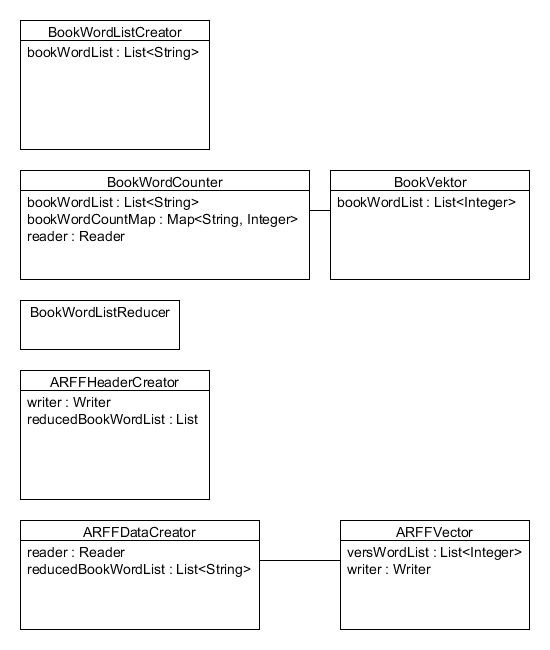
\includegraphics[width=1\textwidth]{Ingo/Bilder/Analyseklassendiagramm_Text2ARFFConverter.png}
\caption{Analyseklassendiagramm Text2ARFFConverter}
\label{fig:Analyseklassendiagramm_Text2ARFFConverter}
\end{figure}

\section{Entwurf Text2ARFFConverter}\label{EntwurfText2ARFFConverter}

In Abbildung \ref{fig:Entwurfsklassendiagramm_Text2ARFFConverter} auf Seite \pageref{fig:Entwurfsklassendiagramm_Text2ARFFConverter} ist das Entwurfsklassendiagramm des Text2ARFF\-Con\-ver\-ters zu sehen.

\begin{figure}[htp]
\centering
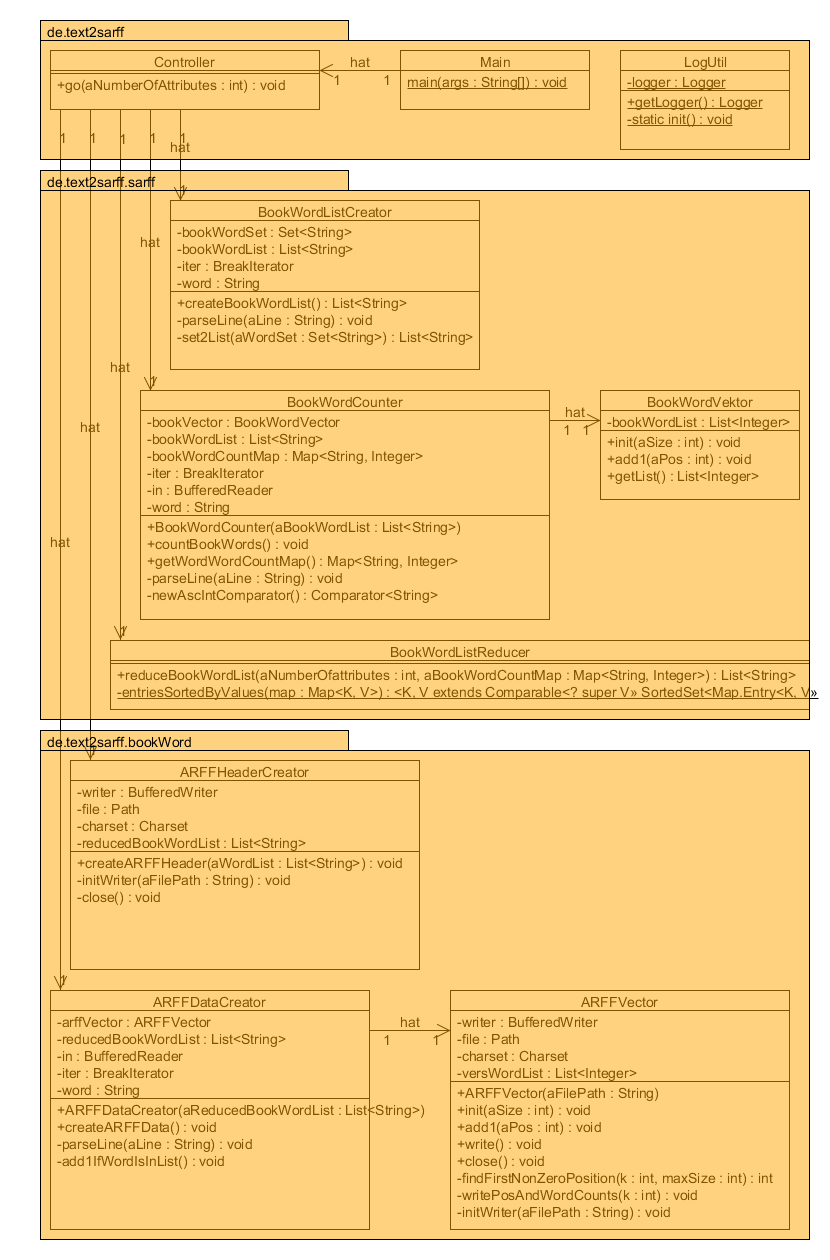
\includegraphics[width=1\textwidth]{Ingo/Bilder/Entwurfsklassendiagramm_Text2ARFFConverter.png}
\caption{Entwurfsklassendiagramm Text2ARFFConverter}
\label{fig:Entwurfsklassendiagramm_Text2ARFFConverter}
\end{figure}

\section{Nach welchen W�rtern sollte geclustert werden?}\label{WelcheWoerter}
Bei Versuchen hat sich gezeigt, dass die Cluster ausgewogener gef�llt sind, wenn die h�ufigsten W�rter gew�hlt werden. Werden die seltensten W�rter gew�hlt, entstehen viele leere Instanzen und es sammeln sich alle Verse in einigen wenigen Clustern und die restlichen Cluster sind fast leer. Wahrscheinlich ist das damit zu begr�nden, dass beim Clustern �hnliche Verse in ein Cluster kommen. Wenn nun aber durch die seltensten W�rter die Verse alle sehr unterschiedlich sind, wird es f�r den Algorithmus schwierig, �hnlichkeiten zu finden. Mit einem Wort, dass nur einmal vorkommt, kann man einen Vers gut von anderen Versen unterscheiden, aber es wird nicht helfen, zu sehen, wo die �hnlichkeiten zu anderen Versen sind. Wenn dagegen W�rter gew�hlt werden, die h�ufig vorkommen, entstehen Cluster, die ausgewogender gef�llt sind. Es kommt mit h�herer Wahrscheinlichkeit zwei Verse in dasselbe Cluster, wenn sie an den selben Positionen die gleichen H�ufigkeiten haben.
\section{H�rden beim Einlesen der ARFF-Datei}\label{Huerden}
Die erzeugte ARFF-Datei wird f�r das AT 900 MB gro�. In Weka kommt auf dem Testrechner beim Einlesen der 900MB gro�en ARFF-Datei die Fehlermeldung "`OutOfMemory"'. Und Weka hat sich darauf hin geschlossen.
In der Konfigurationsdatei RunWeka.ini konnte der Parameter maxheap nur auf h�chstens 1550m gesetzt werden. Wird mehr Platz f�r den heap space angegeben, kommt eine Fehlermeldung von der JVM.
Darauf hin wurde von einem 32Bit-Java auf ein 64Bit-Java gewechselt. Damit verschwanden beide Fehlermeldungen und es konnte der maxheap auf 8000m gesetzt werden.

Wird die ARFF-Datei eingelesen, braucht Weka bzw. die JVM daf�r 6,8 GB Arbeitsspeicher. Auf dem Entwicklungsrechner stehen aber nur 8GB zur Verf�gung. Es wird davon ausgegangen, dass f�r die Anwendung einiger Clusteralgorithmen der restliche Arbeitsspeicher nicht ausreicht und die Geschwindigkeit durch Swapping ausgebremst wird.

Um die Gr��e der ARFF-Datei zu reduzieren, gibt es das Format Sparse ARFF, dass auch gro�e Datenmengen kompakt speichern kann.

Sparse ARFF Dateien sind gew�hnlichen AARF Dateien �hnlich, au�er das Attribute mit dem Wert 0 nicht repr�sentiert werden. Nicht-Null Attribute werden durch die Attributnummer und den Wert angegeben.

Durch Sparse ARFF konnte die Dateigr��e von 900MB auf 4 MB reduziert werden.
Die Datei wird dadurch auch schneller von Weka eingelesen und Weka braucht weniger RAM.
http://wiki.pentaho.com/display/DATAMINING/
\section{SimpleKMeans}\label{SimpleKMeans}
Beim Clustern des AT auf dem Testrechner wurden in Abh�ngigkeit von Attributanzahl und Anzahl der Cluster folgende Ausf�hrungszeiten erzielt.

\begin{figure}[htp]
\centering
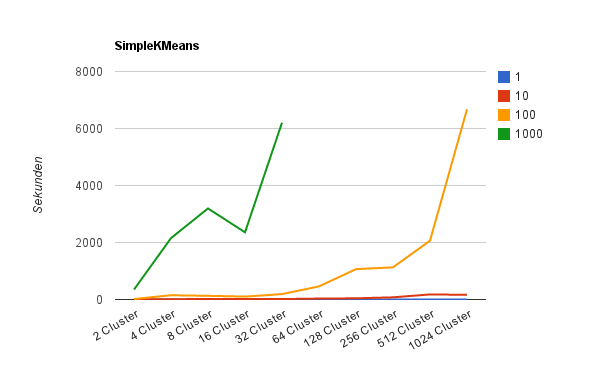
\includegraphics[width=1\textwidth]{Ingo/Bilder/SimpleKMeans.png}
\caption{Ausf�hrungszeiten von SimpleKMeans}
\label{fig:SimpleKMeans}
\end{figure}

In dem Diagramm ist erkennbar, dass die Ausf�hrungszeit steigt, je mehr Attribute und je mehr Cluster es gibt.
Auf einem einzelnen Rechner dauert das Clustern des AT f�r 1000 Attribute und 8 Clustern schon eine knappe Stunde.
F�r mehr Attribute oder mehr Cluster st��t der Testrechner an seine Grenzen.
\section{Weitere Cluster-Algorithmen}\label{weitereClusterAlgorithmen}
Neben SimpleKMeans wurde auch XMeans auf das AT angewandt. Bei XMeans grenzt man die Cluster, die er finden k�nnte mit einer oberen und unteren Schranke ein. XMeans ist ein verleichsweise schneller Clusteralgorithmus, der das AT selbst mit der maximalen Anzahl von 8950 Attributen in 77 Minuten clustert. Dabei findet er drei Cluster. Als obere Schranke wurden zwei und als obere Schranke wurden 16 Cluster angegeben.

Neben SimpleKMeans und XMeans wurden weitere Clustering-Algorithmen angewandt, die aus verschiedenen Gr�nden nicht weiter verfolgt wurden. Das Hierachical Clustering braucht bei nur 5 Attributen mehr als 8GB Arbeitsspeicher um das AT zu clustern. Deswegen konnte dieser Algorithmus auf dem Testrechner nicht ausgef�hrt werden.

Der EM Algorithmus (expectation maximisation) ben�tigt auf dem Testrechner bei zehn Attributen 87 Minuten und findet dabei 7 Cluster. Auf ein clustern mit 100 oder gar 1000 Attributen wurde aus Zeitgr�nden verzichtet.

Der Clusteralgorithmus DBScan bringt beim starten die Fehlermeldung: "`Problem evaluating cluster: null"'. Auch er wurde nicht weiter verfolgt.
\section{geclusterte Instanzen wieder in Verse verwandeln} \label{Text2ClusterFile}
Um aus den geclusterten Instanzen wieder Verse zu machen, die in die jeweils passendes Cluster-Datei geschrieben werden, wird ein Programm namens Text2\-Cluster\-File entwickelt. Das Programm gruppiert anhand der Clusternummer und der Zeilennummer die Verse. So wird erkenntlich, welche Verse wie geclustert wurden. In Abbildung \ref{fig:AnalyseklassendiagrammText2ClusterFile} auf Seite \pageref{fig:AnalyseklassendiagrammText2ClusterFile} ist das Analyseklassendiagramm von Text2\-Cluster\-File zu sehen.

In Abbildung \ref{fig:AnalyseklassendiagrammText2ClusterFile} auf Seite \pageref{fig:AnalyseklassendiagrammText2ClusterFile} ist das Entwurfsklassendiagramm von Text2ClusterFile zu sehen.

\begin{figure}[htp]
\centering
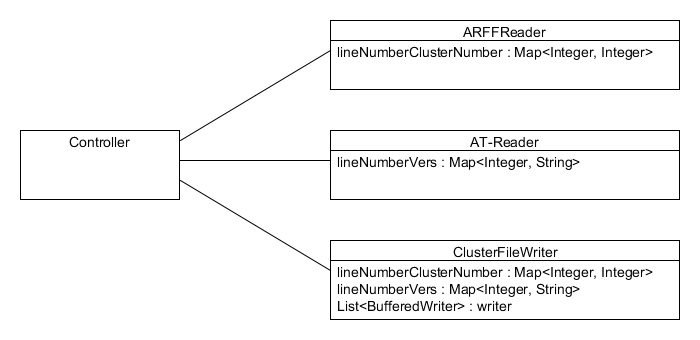
\includegraphics[width=1\textwidth]{Ingo/Bilder/AnalyseklassendiagrammText2ClusterFile.png}
\caption{Analyseklassendiagramm Text2ClusterFile}
\label{fig:AnalyseklassendiagrammText2ClusterFile}
\end{figure}

\begin{figure}[htp]
\centering
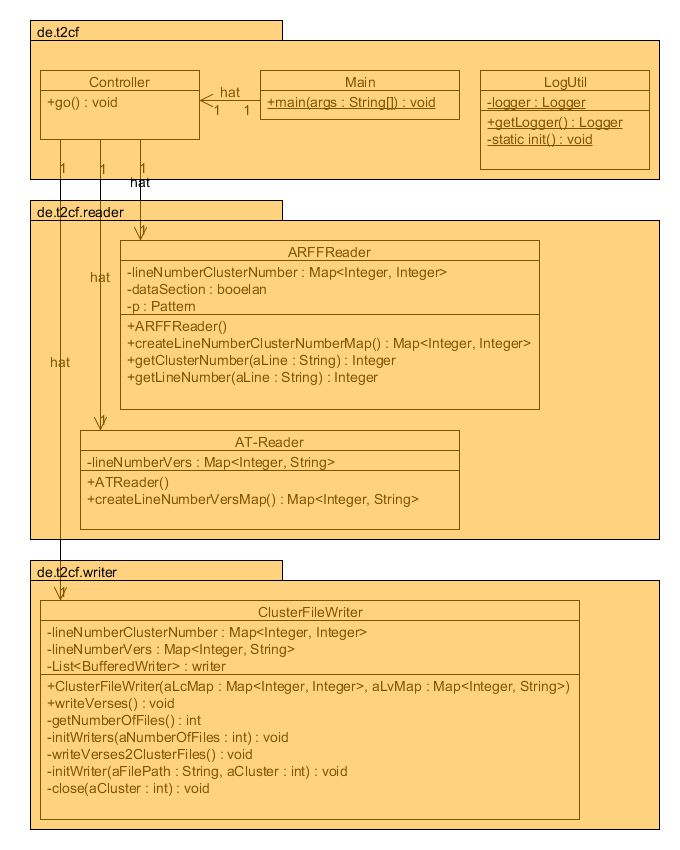
\includegraphics[width=1\textwidth]{Ingo/Bilder/EntwurfsklassendiagrammText2ClusterFile.png}
\caption{Entwurfsklassendiagramm Text2ClusterFile}
\label{fig:EntwurfsklassendiagrammText2ClusterFile}
\end{figure}
\section{AT mit SimpleKMeans geclustert} \label{SimpleKMeansgeclustert}

In Abbildungen \ref{fig:100Attribute1024ClusterCluster15}, \ref{fig:100Attribute1024ClusterCluster49},  \ref{fig:100Attribute1024ClusterCluster61},  \ref{fig:100Attribute1024ClusterCluster86},  \ref{fig:100Attribute1024ClusterCluster554},  \ref{fig:1000Attribute32ClusterCluster4},  \ref{fig:1000Attribute32ClusterCluster5} sowie \ref{fig:1000Attribute32ClusterCluster6} sind Verse zu sehen, die mit SimpleKMeans in ein Cluster gruppiert wurden.

Bei Abbildung \ref{fig:100Attribute1024ClusterCluster49} auf Seite \pageref{fig:100Attribute1024ClusterCluster49} f�llt auf, dass nicht nur in jedem Vers das Wort Herrn vorkommt, und dass auch alle mit der Versnummer 2 anfangen, sondern auch dass oft die Formulierung "`Und er tat, was dem Herrn �bel gefiel"' erscheint.

Bei Abbildung \ref{fig:100Attribute1024ClusterCluster554} auf Seite \pageref{fig:100Attribute1024ClusterCluster554} f�llt auf, dass nicht nur in jedem Vers das Wort "`einen"' vorkommt, sondern dass auch alle mit der Versnummer 1 anfangen.

Auf Abbildung \ref{fig:100Attribute1024ClusterCluster86} auf Seite \pageref{fig:100Attribute1024ClusterCluster86} ist zu sehen, dass hier alle Verse vorkommen, die die Formulierung "`Was aber mehr von ... zu sagen ist und was er getan hat, und seine Macht, und wie er..."' beinhalten.

Wenn es eine hohe Anzahl von Attributen gibt, kann der Cluster-Algorithmus viele W�rter erfassen, mit denen Verse sich �hneln k�nnen. Bei vielen �hnlichen Versen brauch der Algorithmus dann aber auch viele Cluster auf die er die vielen �hnlichen Verse aufteilen kann.

Wenn der Algorithmus nur wenige Attribute aber viele Cluster hat, dann gruppiert er die wenigen Attribute, die ihm zur Verf�gung stehen �ber alle Cluster auf. Wie gut er dabei ist, kann man bei wenigen W�rtern leicht �bersehen, da die meisten W�rter der Verse gar nicht ber�cksichtigt wurden. In den Meisten der 1024 Cluster gibt es aber ein Wort, das alle Verse in diesem Cluster gemeinsam haben.

Es ist zu vermuten, dass wenn alle Attribute genommen werden, die mindestens zwei mal vorkommen, bei steigender Clusteranzahl, die Verse die in einem Cluster vorkommen, zwar im Mittel weniger werden, aber daf�r immer �hnlicher.

\begin{figure}[htp]
\centering
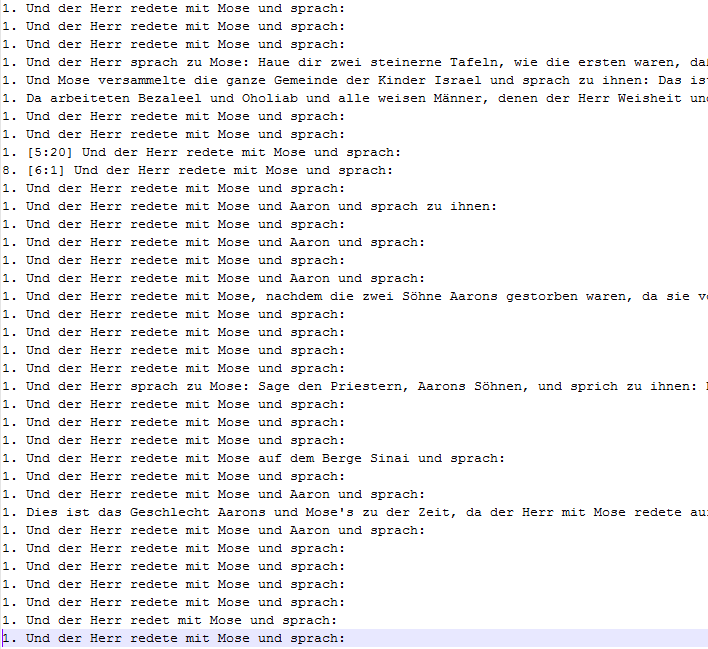
\includegraphics[width=1\textwidth]{Ingo/Bilder/SimpleKMeans100Attr1024Cluster_15.png}
\caption{100 Attribute, 1024 Cluster, Cluster 15}
\label{fig:100Attribute1024ClusterCluster15}
\end{figure}


\begin{figure}[htp]
\centering
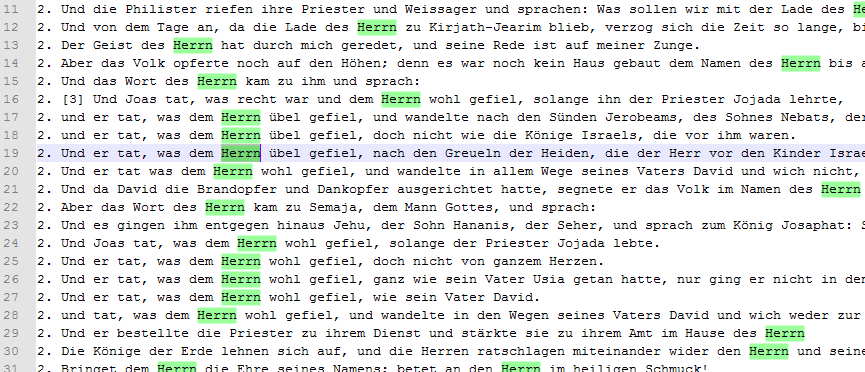
\includegraphics[width=1\textwidth]{Ingo/Bilder/SimpleKMeans100Attr1024Cluster_49.png}
\caption{100 Attribute, 1024 Cluster, Cluster 49}
\label{fig:100Attribute1024ClusterCluster49}
\end{figure}


\begin{figure}[htp]
\centering
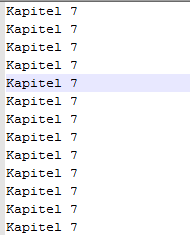
\includegraphics[width=1\textwidth]{Ingo/Bilder/SimpleKMeans100Attr1024Cluster_61.png}
\caption{100 Attribute, 1024 Cluster, Cluster 61}
\label{fig:100Attribute1024ClusterCluster61}
\end{figure}

\begin{figure}[htp]
\centering
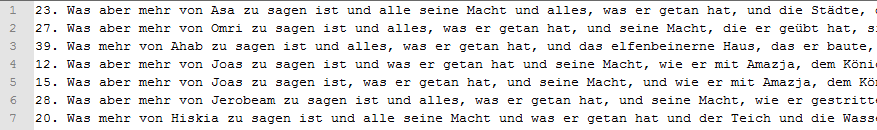
\includegraphics[width=1\textwidth]{Ingo/Bilder/SimpleKMeans100Attr1024Cluster_86.png}
\caption{100 Attribute, 1024 Cluster, Cluster 86}
\label{fig:100Attribute1024ClusterCluster86}
\end{figure}

\begin{figure}[htp]
\centering
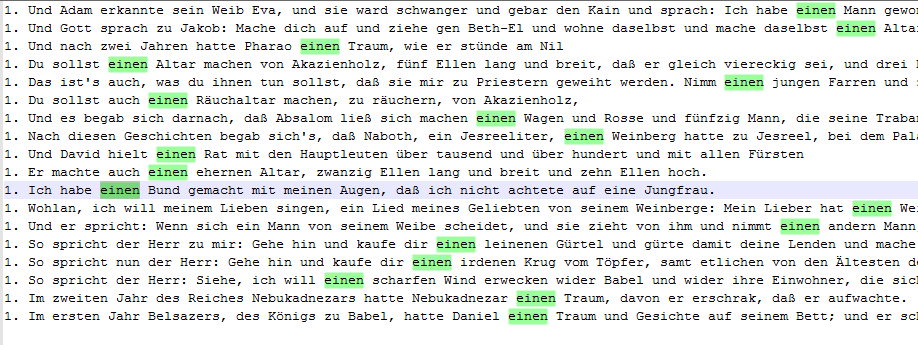
\includegraphics[width=1\textwidth]{Ingo/Bilder/SimpleKMeans100Attr1024Cluster_554.png}
\caption{100 Attribute, 1024 Cluster, Cluster 554}
\label{fig:100Attribute1024ClusterCluster554}
\end{figure}

\begin{figure}[htp]
\centering
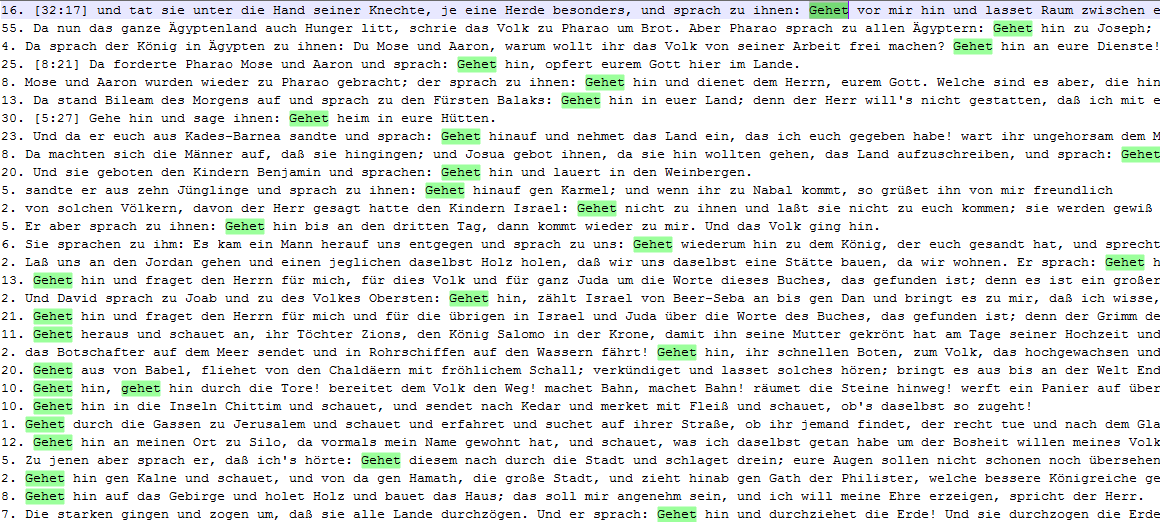
\includegraphics[width=1\textwidth]{Ingo/Bilder/SimpleKMeans1000Attr32Cluster_4.png}
\caption{1000 Attribute, 32 Cluster, Cluster 4}
\label{fig:1000Attribute32ClusterCluster4}
\end{figure}

\begin{figure}[htp]
\centering
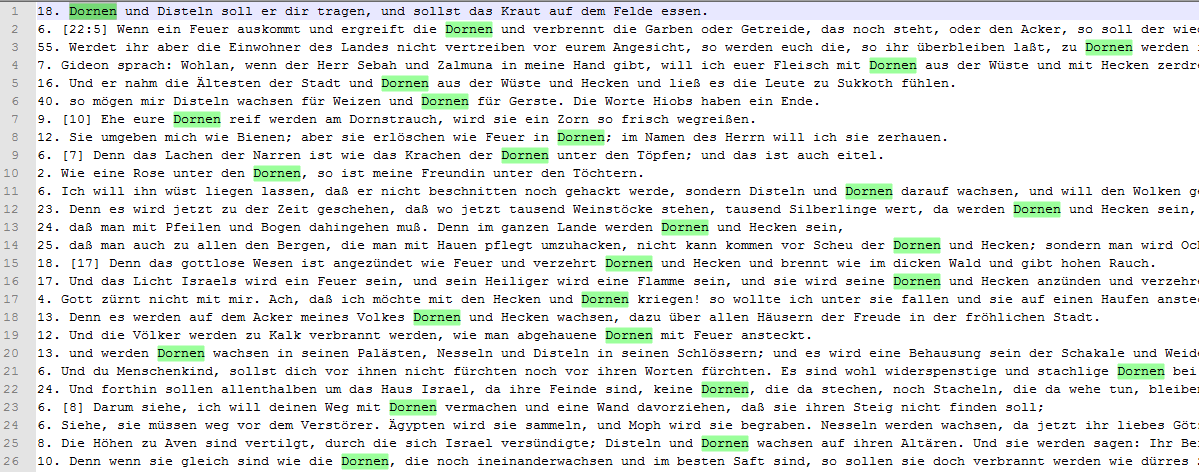
\includegraphics[width=1\textwidth]{Ingo/Bilder/SimpleKMeans1000Attr32Cluster_5.png}
\caption{1000 Attribute, 32 Cluster, Cluster 5}
\label{fig:1000Attribute32ClusterCluster5}
\end{figure}

\begin{figure}[htp]
\centering
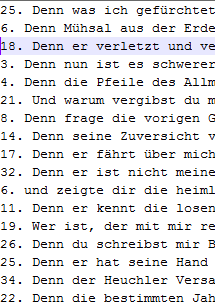
\includegraphics[width=1\textwidth]{Ingo/Bilder/SimpleKMeans1000Attr32Cluster_6.png}
\caption{1000 Attribute, 32 Cluster, Cluster 6}
\label{fig:1000Attribute32ClusterCluster6}
\end{figure}


\begin{figure}[htp]
\centering
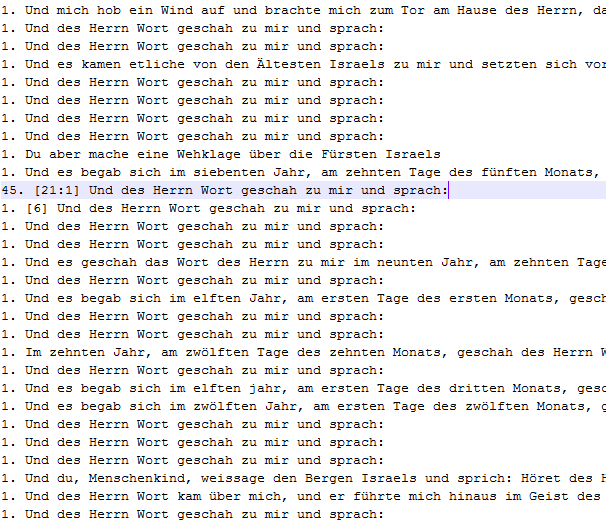
\includegraphics[width=1\textwidth]{Ingo/Bilder/SimpleKMeans1000Attr32Cluster_15.png}
\caption{1000 Attribute, 32 Cluster, Cluster 15}
\label{fig:1000Attribute32ClusterCluster15}
\end{figure}

\section{Zusammenfassung}\label{Zusammenfassung}

\section{Ausblick}\label{Ausblick}
In einem Folgeprojekt k�nnte mit Werkzeugen wie Apache Mahout verwendet werden, mit dem auch verteilt geclustert werden kann.



%\chapter{Theoretische Grundlagen}
%Die f\"{u}r den Untersuchungsgegenstand relevanten Themen, die \"{u}ber die
%grundlegenden Studieninhalte hinausgehen; oft auch anwendungsspezifische Aspekte - %ca. 6 Seiten

%\chapter{Ist-Analyse}
%Welche Defizite sollen mit der Arbeit behoben werden, welche nicht? %Pr\"{a}zisierung
%der Zielstellung - ca. 6 Seiten

%\chapter{L\"{o}sungskonzept}
%Wie sollen die Defizite behoben werden? Methoden, fachliche Auseinandersetzung
%mit alternativen Ans\"{a}tzen und Auffassungen, Systembeschreibung (Architektur,
%Vorgehensmodell, \ldots) - ca. 12 Seiten

%\chapter{Implementierung}
%Umsetzung des L\"{o}sungskonzepts, Begr\"{u}ndung der verwendeten Technologien - %ca. 8
%Seiten

%\chapter{Ergebnisse}
%Objektive Bewertung der vorliegenden L\"{o}sung, diverse Testverfahren,
%Nutzerbefragungen - ca. 4 Seiten

%\chapter{Fazit und Ausblick}
%Zusammenfassung s\"{a}mtlicher Ergebnisse in Bezug auf die Zielerf\"{u}llung und
%Vorschl\"{a}ge f\"{u}r weiterf\"{u}hrende Arbeiten - ca. 2 Seiten

\bibliographystyle{alphadin}
\begin{appendix}
\newpage
\pagestyle{appendixAStyle}
%\chapter{Codebeispiele}
%\begin{lstlisting}[caption=alle Tabellen erstellen, firstnumber=1]{code:TabellenErstellen}
CREATE TABLE "user"
(
  userid bigint,
  name text,
  email text,
  gender text,
  birthday date,
  password text,
  image text
)
WITH (
  OIDS=FALSE
);
ALTER TABLE "user"
  OWNER TO postgres;

CREATE TABLE event
(
  eventid bigint NOT NULL,
  creatorid bigint,
  date date,
  eventname text,
  occasion text,
  location text,
  lon double precision,
  lat double precision,
  description text,
  numbermaleconfirmed int,
  numberfemaleconfirmed int
)
WITH (
  OIDS=FALSE
);
ALTER TABLE event
  OWNER TO postgres;

CREATE TABLE message
(
  messageid bigint,
  eventid bigint,
  senderid bigint,
  recipientid bigint,
  textmessage text,
  date date
)
WITH (
  OIDS=FALSE
);
ALTER TABLE message
  OWNER TO postgres;

CREATE TABLE participation
(
  participationid bigint,
  userid bigint,
  eventid bigint
)
WITH (
  OIDS=FALSE
);
ALTER TABLE participation
  OWNER TO postgres;
\end{lstlisting}

\begin{lstlisting}[caption=Datenimport �ber COPY, firstnumber=1]{code:COPY}
COPY public.Event (eventid, creatorid, date, eventname, occasion, location, lon, lat, description, numbermaleconfirmed, numberfemaleconfirmed) From 'C:\Event.txt' DELIMITER ';';
COPY public.Message (messageid, eventid, senderid, recipientid, textmessage, date) From 'C:\Message.txt' DELIMITER ';';
COPY public.Participation (participationid, userid, eventid) From 'C:\Participation.txt' DELIMITER ';';
COPY public.User (userId, name, email, gender, birthday, password, image) From 'C:\User.txt' DELIMITER ';';
\end{lstlisting}


\begin{lstlisting}[caption=Prim�r- und Fremdschl�ssel hinzuf�gen, firstnumber=1]{code:PrimaryForeignKeys}
ALTER TABLE public.event ADD PRIMARY KEY (eventid);
ALTER TABLE public.message ADD PRIMARY KEY (messageid);
ALTER TABLE public.participation ADD PRIMARY KEY (participationid);
ALTER TABLE public.user ADD PRIMARY KEY (userid);

ALTER TABLE event ADD CONSTRAINT event_creatorid FOREIGN KEY (creatorid) REFERENCES public.user (userid) MATCH FULL;
ALTER TABLE message ADD CONSTRAINT message_eventid FOREIGN KEY (eventid) REFERENCES event (eventid) MATCH FULL;
ALTER TABLE message ADD CONSTRAINT message_senderid FOREIGN KEY (senderid) REFERENCES public.user (userid) MATCH FULL;
ALTER TABLE message ADD CONSTRAINT message_recipientid FOREIGN KEY (recipientid) REFERENCES public.user (userid) MATCH FULL;
ALTER TABLE participation ADD CONSTRAINT participation_userid FOREIGN KEY (userid) REFERENCES public.user (userid) MATCH FULL;
ALTER TABLE participation ADD CONSTRAINT participation_eventid FOREIGN KEY (eventid) REFERENCES event (eventid) MATCH FULL;
\end{lstlisting}


\begin{lstlisting}[caption=Indexe auf Spalten legen, firstnumber=1]{code:Indexe}
CREATE INDEX event_creatorid ON public.event(creatorid);
CREATE INDEX message_eventid ON public.message(eventid);
CREATE INDEX message_senderid ON public.message(senderid);
CREATE INDEX message_recipientid ON public.message(recipientid);
CREATE INDEX participation_userid ON public.participation(userid);
CREATE INDEX participation_eventid ON public.participation(eventid);

CREATE INDEX event_date ON public.event(date);
CREATE INDEX event_eventname ON public.event(eventname);
CREATE INDEX event_occasion ON public.event(occasion);
CREATE INDEX event_location ON public.event(location);
CREATE INDEX event_lon ON public.event(lon);
CREATE INDEX event_lat ON public.event(lat);
CREATE INDEX event_numbermaleconfirmed ON public.event(numbermaleconfirmed);
CREATE INDEX event_numberfemaleconfirmed ON public.event(numberfemaleconfirmed);

CREATE INDEX message_textmessage ON public.message(textmessage);
CREATE INDEX message_date ON public.message(date);

CREATE INDEX user_name ON public.user(name);
CREATE INDEX user_email ON public.user(email);
CREATE INDEX user_gender ON public.user(gender);
CREATE INDEX user_birthday ON public.user(birthday);
\end{lstlisting}
\end{appendix}

\newpage
\chapter{Arbeitsaufteilung}


\begin{table}[h] \begin{flushleft}  \begin{tabular}{|l||c|c|c|c|c|c|}
\hline
\textbf{Arbeit}		&	\textbf{C. Ochmann}	& \textbf{I. K�rner}  \\ \hline \hline
Abstract   	      &                     & 0       \\
Einleitung  &                             		      & ~\ref{Einleitung} \\
Aufgabenstellung&                                  & ~\ref{Aufgabenstellung}  \\
Forschungsgegenstand&                              & ~\ref{RelevanzDesForschungsgegenstandes} \\ 
akt. Wissensstand&                                      & ~\ref{DerAktuelleWissensstand}  \\ 
Testrechner&                                      & ~\ref{Testrechner}  \\ 
Der Aufbau des AT&                                      & ~\ref{AufbauAT}  \\ 
ARFF&                                      & ~\ref{ARFF}  \\ 
Clustering-Verfahren&       ~\ref{Clustering}                                &  \\ 
Partitionierende Verfahren&       ~\ref{Partitionierende}                                &  \\ 
Austauschverfahren mit Zielfunktion&       ~\ref{Austausch}                        &  \\ 
Minimaldistanz-Verfahren&       ~\ref{Minimal}                        &  \\ 
Minimaldistanz-Verfahren&       ~\ref{Minimaldistanz}                        &  \\ 
k-Means-Verfahren&       ~\ref{kmeans}                        &  \\ 
EM-Algorithmus&       ~\ref{em}                        &  \\ 
DBSCAN&       ~\ref{dbscan}                        &  \\ 
Hierarchische-Verfahren&       ~\ref{Hierarchische}                        &  \\ 
Agglomerative-Verfahren&       ~\ref{Agglomerative}                        &  \\ 
Wie AT in das ARFF-Format �berf�hren?&                                      & ~\ref{ATzuARFF}  \\ 
Analyse Text2ARFFConverter&                                      & ~\ref{AnalyseText2ARFFConverter}  \\ 
Entwurf Text2ARFFConverter&                                      & ~\ref{EntwurfText2ARFFConverter}  \\ 
Nach welchen W�rtern clustern?&                                      & ~\ref{WelcheWoerter}  \\ 
H�rden beim Einlesen der ARFF-Datei&                                      & ~\ref{Huerden}  \\ 
SimpleKMeans&                                      & ~\ref{SimpleKMeans}  \\ 
Weitere Cluster-Algorithmen&                                      & ~\ref{weitereClusterAlgorithmen}  \\ 
Instanzen in Verse verwandeln&                                      & ~\ref{Text2ClusterFile}  \\ 
AT mit SimpleKMeans geclustert&                                      & ~\ref{SimpleKMeansgeclustert}  \\ 
Zusammenfassung&         																& ~\ref{Zusammenfassung} \\ 
Ausblick&        																					 & ~\ref{Ausblick} \\ 
\hline \hline
\end{tabular} \end{flushleft} \caption{Aufteilung} \end{table}



\newpage
\chapter{Eigenst�ndigkeitserkl�rung}
Hiermit erkl�re ich, dass ich diese Arbeit selbst�ndig verfasst habe. Mir ist bekannt, dass jede Form des Plagiats mit der Note 5 (Betrugsversuch) bewertet wird.

\begin{tabular}{@{}p{6.0cm}p{6.0cm}}	  		  		 	
	  		 & \\
	  		 & \\
				  			\textbf{Ochmann, Christof} &               Unterschrift:\\				 
				 &\\
				 & \\
				  			\textbf{K�rner, Ingo}   	&                     Unterschrift:\\			
\end{tabular}
\end{document}
